\section{Einführung}

In der Computergrafik ist die Erzeugung eines Dreiecksnetzes eine gängige Methode zur Generierung von 3D-Modellen. Diese Modelle können in Topologie und Geometrie unterteilt werden. Für die Geometrie werden verschiedene Attribute benötigt. 
So werden die Positionen, die Normalenvektoren und Texturekoordinaten/Farbwerte für jeden Punkt des Dreiecksnetzes in single-precision floating point values (32 Bit Gleitkommazahlen) gespeichert. 
Für die korrekte Annordung und Reihenfolge der Knotenpunkte ist die Topologie zuständig. 
Dabei ist die Datenkompression ein entscheidendes Thema. 
In einer Welt, in der digitale Daten schon lange ein wichtiges Thema sind, und dennoch immer weiter an Bedeutung gewinnen, ist die effiziente Speicherung und Übertragung ein wichtiger Gesichtspunkt.
3D Modelle werden so gut wie überall benötigt. 
Videospiele und Animationsserien wären ohne nicht vorstellbar. 
Architekten können ihre Ideen auch ohne Bleistift auf das Papier (oder den Bildschirm) bringen.
Künstler wollen Modelle erschaffen, die den Eindruck gewinnen wollen, realitätsgetreu zu sein. 
Die Folge davon ist, dass diese Modelle stetig komplexer werden, und somit ein größerer Speicheraufwand benötigt wird. 
Um dem entgegenzuwirken, werden Methoden verwendet, diese digitalen Informationen zu komprimieren. \newline

\subsection{Geschichtliche Ausarbeitung Thema Datenkompression}
\label{subsec:main_kompression}
Ursprünglich zur Repräsentation von Daten entwickelt, wurde der Morse Code zu einem der wichtigsten Werkzeuge für die Kommunikation des 19. Jahrhunderts. 
Bestehend aus zwei Grundbausteinen, einem kurzen und einem langen Signal, konnten einzelne Buchstaben kodiert werden. 
Erweitert man dieses Alphabet mit einem weiteren \glqq Symbol\grqq\, einer Pause, die zwischen einzelnen Signalsequenzen eingelegt wird, können ganze Sätze übermittelt werden. 
Das bekannteste Werkzeug für den Morse Code ist der Telegraf, mit dem diese Signale über weite Strecken übertragen werden konnten.
Die Erfindung des Morsecodes findet im 21. Jahrhundert nicht nur seinen Zweck in dramatischen Momenten des in Film und Fernsehens. 
Es war zeitgleich ein früher und großer Meilenstein und Wegbegleiter für die Kompression einer Datenquelle (in diesem Fall das Alphabet). 
Durch Untersuchungen einer großen Anzahl an Literatur kann eine Buchstabenhäufigkeit berechnet werden. 
Diese sagt aus, wie wahrscheinlich es ist, welcher Buchstabe in einem Text folgt, ohne den aktuellen Kontext, in Form von vorgehenden Buchstaben, zu betrachten.
Da die Wahrscheinlichkeit eines Zeichens abhängig vom Alphabet ist, sollten diese nicht übergreifend verwendet werden. 
So sind die Buchstaben \glqq E\grqq\ und \glqq T\grqq\ die Buchstaben des englischen Alphabets, welche die höchste Auftrittswahrscheinlichkeit besitzen, während sich im deutschen Alphabet der Buchstabe \glqq E\grqq\ von der Masse abhebt.
%Datenkompression problem ausführen: durch ein stop Signal geht eine wichtige Eigenschaft verloren (eventuell binär)
Der Morse Code hat gezeigt, welchen Nutzen die Kompression von Information beinhaltet.
Zu Kriegszeiten hat dieser eine effiziente und schnelle Übermittlung von Informationen ermöglicht.
Dadurch konnte in Krisenmomenten schnell reagiert werden, um so größeren Katastrophen frühzeitig abzuwenden, aber leider auch zu verursachen.

\subsubsection*{Der Ist-Stand}
Springen wir in die heutige Zeit sehen wir die Auswirkung von komprimierten Daten.
Die meisten Menschen denken an JPEGs und PNGs, wenn sie an digitale Bilder denken.
Bekanntere Videoformate sind MP4, AVI und FLV.
Bei all diesen Formaten handelt es sich um komprimierte Rohdaten.
Das Filesystem eines jeden relevanten Betriebssystems komprimiert beim Speichern von Daten diese automatisch.
Zusätzlich dazu besteht noch die Möglichkeit, seine Daten manuell zu komprimieren mithilfe von Programmen wie 7Zip, WinRar oder WinZip.
Datenkompression kann in so gut wie allen Bereichen angetroffen werden.
Und die Gründe dafür sind simpel.
Speicherplatz ist teuer, und das Ressourcenmanagement wird deutlich vereinfacht, wenn die benötigte Hardware minimiert wird.
Betrachten wir das Streamen von Daten auf dem Beispiel des größten Videostreaming Dienstes Youtube.
Laut Statistiken werden pro Minute hunderte Stunden an Videomaterial hochgeladen Tendenz steigend (Abb.~).
\begin{figure}[htb]
  \centering  
  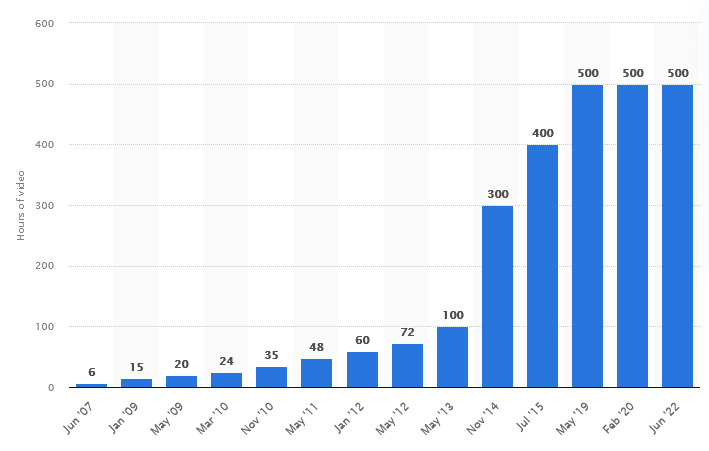
\includegraphics[scale=0.8]{Bilder/youtube_statistik.png}
  \caption[Youtube Statistik]{\textbf{Anzahl der Youtube Videos} Die Anzahl an Minuten die auf Youtube hochgeladen werden.
  Abbildung von Statista: https://www.statista.com/statistics/259477/hours-of-video-uploaded-to-youtube-every-minute/ }
  \label{fig:youtube}
\end{figure}
Um die Unmengen an Videos zu speichern, benötigt Google riesige Serverfarmen, die auf dem gesamten Globus verstreut sind.
Eine genaue Zahl ist der Öffentlichkeit nicht bekannt, es steht jedoch außer Frage, dass diese nochmal um einiges höher ausfällt, würde es keine Verfahren zur Datenkompression geben. \newline

Ein weiterer Gesichtspunkt ist der eigentliche Nutzen von Youtube, dem Streamen von Videos.
Um ein Video sehen zu können, muss dieses von dem Youtube Server, zum Nutzer, dem Client übertragen werden.
Durch die Komprimierung der Quelldateien sind die zu übertragenden Daten schon geschrumpft.
Es können jedoch noch weitere Schritte absolviert werden, um die Daten für den Nutzer besser zugänglich zu machen.
Dazu werden Verfahren wie Trancoding, Transsizing und Transrating verwendet.
Transcoding beschreibt den Prozess, ein bereits komprimiertes Videoformat in ein anderes, eventuell für den Client besser zugeschnittenes Videoformat zu komprimieren.
Das sollte jedoch nicht zu oft angewendet werden, da die Qualität beim wiederholten dekomprimieren und komprimieren verloren geht, sollten die Verfahren verlustbehaftet sein. \newline
In vielen Fällen kann die originale Auflösung vom Endgerät nicht abgespielt werden, und wird deshalb von diesem auf eine niedrigere Auflösung skaliert.
Beispielsweise wenn das Endgerät lediglich 1080p auflösen kann, aber ein Video in 4K Auflösung gestreamt werden soll.
Trotzdem werden die vollen Daten des Videoformats empfangen.
Um diese Verschwendung von Bandbreite zu sparen, wird Transsizing verwendet.
Die originalen Daten werden in eine kleinere Auflösung skaliert, und anschließend übertragen. \newline
Um die Bitrate zu minimieren wird Transrating verwendet.
So kann die Auflösung beibehalten werden bei jedoch geringere Bitrate.
Die Verfahren zur Minimierung des Datenstroms hören sich zunächst sehr mächtig an, sind jedoch mit Vorsicht zu genießen.
Der Vorgang ist nämlich Verlustbehaftet und kann bei zu starker Nutzung zu Artefakten führen.
Dafür ermöglicht es jedoch Menschen, deren Internetzugang ein Abspielen in hoher Qualität nicht zulässt, den Streaming Anbieter zu nutzen.

Der Ursprung der Datenkompression ist dementsprechend der Weiterentwicklung des Morse Codes zurückzuführen. 

TODO

\subsection{Steigende Komplexität}
\label{subsec:steigende_komplexität}
Um die Realität bestmöglich darzustellen, werden Modelle stetig detailreicher, wodurch die Anforderungen an der Hardware steigen. In einer komplexen Szene können mehrere Millionen Dreiecke sichtbar sein, die je nach Anwendung, in Echtzeit gerendert werden müssen. Der Wunsch nach realistischeren Modellen in der Animationsfilm und Videospielbranche hat die Dreiecksanzahl von 3D Modellen in die Höhe schießen lassen. 

\subsection{Ziel der Arbeit}
